% Proc jsem delali rozhodnuti kdyz vznikala ta implementace.
\chapter{Analýza}
\label{chap:analysis}
V této kapitole prozkoumáme jaké rozhodnutí byla udělána během implementace a odůvodníme jejich zvolení.

% Prvně nahlédneme na abstrakční vrstvu a poté na samotnou hru.

\section{Volba frameworku/enginu pro hru}
Chceme vytvořit hru a s její pomocí porovnat výkon ECS knihoven. Implementace se tedy bude skládat ze dvou částí a to samotné hry a měření, které pomocí naší hry bude měřit výkon jednotlivých ECS knihoven.

Nyní provedeme volbu engninu/frameworku, který použijeme pro naši hru. Pro tuto volbu si nejprve rozeberme požadavky, které od engninu/frameworku chceme:

\begin{enumerate}
    \item \textbf{Podpora pro programovací jazyk C\#:} V sekci~\ref{sec:ecs-libs} jsme si uvedli, že se zaměříme na knihovny pro programovací jazyk C\#. Proto tento programovací jazyk budeme chtít použít pro naši hru.
    \item \textbf{Podpora pro 2D hry s pohledem shora:} Tento požadavek vyplývá ze specifikace hry, konkrétně ze sekce~\ref{sec:game-spec}.
    \item \textbf{Možnost spouštět hru vícekrát po sobě a z jiného C\# projektu:} Kromě naší hry budeme mít také měření, které pomocí naší hry změří výkon různých ECS knihoven. Jak naše hra tak i naše měření budou samostatné C\# projekty. Od frameworku/enginu budeme vyžadovat aby nám umožnil spouštět hru vícekrát po sobě s různými implementacemi abstrakční vrstvy z našeho měření, které je v jiném C\# projektu než naše hra.    
\end{enumerate}

V přehledu~\cite{SteamDB} technologií používaných hrami v herním obchodě Steam~\cite{Steam} je možné nahlédnout, že mezi nejpopulárnější herní enginy/frameworky pro C\# patří Unity~\cite{Unity}, Godot~\cite{Godot} a Microsoft XNA Framework.

Unity a Godot jsou velké herní enginy s vlastním editorem. Oba dva podporují 2D hry s pohledem shora. Ovšem tyto enginy odstiňují uživatele od některých nízkoúrovňových částí implementace a přebírají kontrolu na C\# projektem. Bylo by pro nás problematické s nimi splnit třetí požadavek (Možnost spouštět hru vícekrát po sobě a z jiného C\# projektu).

Microsoft XNA Framework je pouze knihovna tříd bez vlastního editoru. Tento framework je vhodný pro 2D hry s pohledem shora a oproti herním enginům Unity a Godot tento framework volí nízkoúrovňoví přístup, díky kterému uživatel není odstíněn od nízkoúrovňových částí implementace a má plnou kontrolu nad projektem. Tím pádem tento framework splňuje všechny naše požadavky.

Ačkoliv by tento framework byl vhodným kandidátem, bohužel již není delší dobou firmou Microsoft podporován. Ale jelikož se jednalo o velice populární herní framework, tak po skončení jeho podpory vzniklo několik open source reimplementací, které v podpoře a vývoji tohoto herního frameworku pokračují. Mezi nejpopulárnější z nich patří FNA~\cite{FNA} a MonoGame~\cite{MonoGame}. Oba tyto frameworky mají téměř identické API, my pro implementaci naši hry zvolíme MonoGame z důvodů osobní preference autora.

% analyza abstrakce
\section{Abstrakční vrstva}
\label{section:abstract-layer-analysis}
Abstrakční vrstva pro nás je důležitá, jelikož chceme aby naše hra byla nezávislá na konkrétní ECS knihovně. Program jako takový bude pracovat namísto ECS knihovny pouze s touto abstrakční vrstvou. Pro každou ECS knihovnu, kterou budeme měřit bude nutné vytvořit implementaci této vrstvy. K volbě konkrétní ECS knihovny dojde před spuštěním programu.

\subsection{Rozhraní ECS knihoven}
Pro návrh abstrakční vrstvy bude nejprve nutné rozebrat jak jsou jednotlivé prvky ECS reprezentovány při jejich implementaci. Krom základních členů, jako jsou \textit{entity}, \textit{komponenty} a \textit{systémy}, si představíme ještě \textit{world} a \textit{query}.

\begin{enumerate}
    \item \textbf{\textit{Component}:} \textit{Komponenty}, jako takové, bývají často reprezentovány třídou nebo strukturou. Jak již bylo zmíněno v úvodu, \textit{komponenty} obsahují pouze data, nikoliv žádnou logiku. Proto tyto třídy a struktury neobsahují žádné metody.

    \item \textbf{\textit{Entity}:} \textit{Entita} by, podobně jako v návrhovém vzoru Component, mohla být reprezentována jako kolekce svých \textit{komponent}. Ovšem to se v praxi nedělá, namísto toho se používá řešení, které vede k lepšímu výkonu. Většina ECS implementacích reprezentuje \textit{entity} pouze jako jednoduchý identifikátor a jednotlivé \textit{komponenty} jsou na \textit{entity} mapovány skrze \textit{world}.

    \item \textbf{\textit{World}:} \textit{World} je spravce \textit{entit} a \text{komponent}. Tento správce slouží jako kontejner pro všechny \textit{entity} a \textit{komponenty} v herním světě. Jeho rozhraní nabízí funkce, pomocí niž je možné vytvářet a mazat jednotlivé \textit{entity}. Často obsahuje také funkce pro přidávání a odebírání \textit{komponent} jednotlivým \textit{entitám}.

    Některé ECS implementace reprezentují \textit{entity} pomocí malé struktury, obsahující identifikátor dané \textit{entity} společně s referencí na \textit{world} do kterého patří. To umožňuje mít na této struktuře bohaté rozhraní s funkcemi pro přidávání a odebírání \textit{komponent}.

    \item \textbf{\textit{System}:} Reprezentace \textit{systémů} se v jednotlivých ECS implementacích dost liší. Některé vyžadují aby \textit{systém} byl třída dědicí od abstraktního předka, jiné zase volí opačný extrém a dovolují \textit{systém} reprezentovat téměř jakkoliv. Navzdory velkým odlišnostem se ve velkém počtu ECS implementací často objevuje objekt, který mohou používat jednotlivé systémy pro iterování entit s určitou množinou komponent.

    \item \textbf{\textit{Query}:} \textit{Query} je objekt, který lze použít pro iterování \textit{entit} s určitou množinou \textit{komponent}. Pro jeho vytvoření je většinou nutné poskytnou informaci, nad jakými typy \textit{komponent} bude \textit{query} pracovat. Je například možné mít \textit{query}, které pracuje nad \textit{komponentami} \verb|Movement| a \verb|Position|. Takové \textit{query} by pak bylo schopné iterovat nad všemi \textit{entitami} co mají \textit{komponenty} \verb|Movement| a \verb|Position|. Pomocí tohoto \textit{query} by bylo možné implementovat \verb|MovementSystem|, který by řídil logiku pohybu.
\end{enumerate}

Pro reprezentaci \textit{systémů} v naší abstrakční vrstvě bude nejprve nutné si přiblížit jak jednotlivé ECS knihovny reprezentují \textit{systémy}. Jak již bylo zmíněno, reprezentace \textit{systémů} se v jednotlivých ECS knihovnách dost liší. Významný rozdíl spočívá ve způsobech, jakými iterují \textit{entity}. Tyto způsoby se dají rozdělit do tří kategorií, kde každá kategorie obsahuje tři způsoby. Nyní si rozebereme jednotlivé kategorie a způsoby. Vždy prvně představíme pseudokód pro způsoby z této kategorie a poté danou kategorii popíšeme.

\subsubsection{1. kategorie}

\begin{enumerate}
    \item \verb|Query((entity) => { /**/ })|
    \item \verb|Query((component1, component2) => { /**/ })|
    \item \verb|Query((components1[], components2[]) => { /**/ })|
\end{enumerate}

Způsoby z této kategorie mají většinou definovanou metodu \verb|Query| (neplést s \textit{query} jako objektem pro iterování \textit{entit}). Tato metoda bývá často implementována na \textit{query} nebo na \textit{world}. Této metodě se předává lambda funkce, která je v případě 1 volána na každou iterovanou \textit{entitu}, v případě 2 volána na množinu žádoucích instancí \textit{komponent} každé iterované \textit{entity}, v případě 3 volána na množinu polí, které obsahují žádoucí instance \textit{komponent} a kde jako index do těchto polí lze použít identifikátor příslušné \textit{entity}.

\subsubsection{2. kategorie}

\begin{enumerate}
    \setcounter{enumi}{3}
    \item \verb|void Update(entity) { /**/ }|
    \item \verb|void Update(component1, component2) { /**/ }|
    \item \verb|void Update(components1[], components2[]) { /**/ }|
\end{enumerate}

Způsoby z druhé kategorie vyžadují aby \textit{systém} byl třída, dědicí od rozhraní nebo předka. Toto rozhraní nebo předek nabízí abstraktní metodu \verb|Update|, kterou je nutné přetížit. Při iteraci je v případě 4 metoda \verb|Update| volána na každou iterovanou \textit{entitu}, v případě 5 na množinu žádoucích instancí \textit{komponent} každé iterované \textit{entity}, v případě 6 na množinu polí, které obsahují žádoucí instance \textit{komponent} a kde jako index do těchto polí lze použít identifikátor příslušné \textit{entity}.

\subsubsection{3. kategorie}

\begin{enumerate}
    \setcounter{enumi}{6}
    \item \verb|foreach (entity in entities) { /**/ }|
    \item \verb|foreach ((component1, component2) in entities) { /**/ }|
    \item \verb|for (int i = 0; i < entitiesCount; i++)|\\\verb|{ components1[i], components2[i], /**/ }|
\end{enumerate}

Třetí kategorie nabízí kolekce nebo iterátory, které lze iterovat. Tyto kolekce nebo iterátory lze získat voláním příslušné funkce na \textit{world} nebo \textit{query}. V případě 7 tato kolekce nebo iterátor obsahuje všechny \textit{entity}, které chceme iterovat. V případě 8 tato kolekce nebo iterátor obsahuje n-tice žádoucích instancí \textit{komponent} každé iterované \textit{entity}. V případě 9 je namísto kolekce použita množina polí, které obsahují žádoucí instance \textit{komponent} a kde jako index do těchto polí lze použít identifikátor příslušné \textit{entity}.

\subsection{Inlinování funkce}
Při pohledu na způsoby pro iterování entit z minulé sekce přirozeně vyplývá pro každou entitu zavolat funkci (konkrétně na místě komentáře \verb|/**/|), která danou entitu zpracuje. Ovšem volání funkce nás stojí čas. Tento čas není moc velký a je většinou zanedbatelný s porovnáním s časem vykonávání funkce samotné. Ovšem my bychom chtěli volat funkci pro každou žádoucí entitu a v případě, že by tato funkce byla jednoduchá (její vykonání by trvalo malé množství času), tak se jednotlivé časy volání této funkce nasčítají a naše řešení by vedlo ke ztrátě na výkonu. Předtím než si navrhneme samotné systémy, bude nutné si tuto problematiku více přiblížit.

Některé ECS knihovny se snaží tomuto problému předejít tím, že namísto toho aby jejich systémy přijímali funkci, kterou zavolají na každou entitu, poskytnou uživateli kolekce nebo iterátory, které si uživatel sám zpracuje. Tím se volání funkce vyhnou úplně. Znamená to tedy, že náš způsob ublíží na výkonu pouze některým knihovnám a to by mělo vliv na naše porovnání. Konkrétně se jedná o způsoby 3, 6, 7, 8 a 9 z minulé sekce.

JIT používá optimalizaci, při které se nahradí místo volání funkce samotným obsahem dané funkce. Díky tomu může být volání takovéto funkce zadarmo. Konkrétně se jedná o takzvané \textit{inlinování funkce} (\textit{inline expansion}). Ovšem JIT tuto optimalizaci ne vždy provede, jelikož v některých případech se to nevyplatí nebo to dokonce udělat nemůže.

Pro více informací o tom kdy dochází a nedochází k \textit{inlinování funkcí}, je možné nahlédnout do článků od Davida Notaria~\cite{Notario_2004} a Vance Morrisona~\cite{Morrison_2008}. Konkrétně pro nás jsou důležité dva body.

\begin{enumerate}
    \item K \textit{inlinování funkce} nedojde, pokud se jedná o virtuální volání funkce.
    \item K \textit{inlinování funkce} nedojde, pokud je kód dané funkce příliš velký.
\end{enumerate}

Je nutné zmínit, že tyto články jsou již starší a nyní jsou pravidla pro inlinování méně přísná. Například JIT je schopný v některých případech provést \textit{inlinování funkce} i přes to, že se jedná o virtuálního volání funkce.

\subsection{Reprezentace systémů}
Jak již bylo v minulé sekci naznačeno, každý systém bude mít tedy funkci, kterou bude volat na každou entitu. Zároveň každý systém iteruje jednotlivé entity jiným způsobem. Systémy tedy budeme reprezentovat tím, že si pořídíme dva typy.

\begin{enumerate}
    \item \textbf{\texttt{EntityProcessor}:} Tento typ bude mít na sobě již zmiňovanou funkci pro zpracování jedné entity. Nazvěme ji \verb|Process|.
    \item \textbf{\texttt{IECSSystem}:} Jedná se o rozhraní. Pro každou ECS knihovnu, kterou budeme chtít měřit, implementujeme třídu, která hude dědit od tohoto rozhraní. Toto rozhraní bude nabízet metodu \verb|Update| ve které implementujeme iteraci přes jednotlivé entity. Každá instance takového systému bude mít také instanci \verb|EntityProcessor|, jejíž metodu \verb|Process| při iteraci zavolá na jednotlivé entity.
\end{enumerate}

Tím jsme vyřešili různé reprezentace systému, ale ještě zbývá problém s \textit{inlinováním funkce}. Vyřešíme to tím, že jednotlivé \verb|EntityProcessor| budou struktury, které budou dědit od rozhraní \verb|IEntityProcesor|. Instance systému poté přijme typ konkrétního \verb|EntityProcessor| jako generický argument.

Nyní si vysvětlíme proč je pro nás důležité, že jednotlivé \verb|EntityProcessor| jsou struktury.

Při první konstrukci generického typu, který má hodnotový datový typ jako parametr se vytvoří specializace dané třídy, ve které je daný parametr nahrazen daným typem. Je nutné poznamenat, že k tomuto dochází pouze v případě dosazení hodnotového datového typu (struktury jsou hodnotové datové typy). V případě referenčních datových typů se vytváří pouze jedna jediná specializace ve které je daný argument nahrazen typem \verb|object|. Pro více informací o tomto procesu je možné nahlédnout do článku \textit{Generics in the runtime (C\# programming guide)}~\cite{GenericsInTheRuntime} od firmy Microsoft.

Při použití konkrétního systému, kterému předáme jako generický argument jeden z \verb|EntityProcessor|, dojde tedy k výše zmíněnému procesu. Konkrétně dojde k vytvoření specializace pro již zmiňovanou metodu \verb|Update|. Tato specializace iteruje jednotlivé entity a na každé z nich volá metodu \verb|Process| na konkrétním \verb|EntityProcessor|. Na tomto volání může JIT provést \textit{inlinování}.

Může se stát, že metoda \verb|Process| na konkrétním \verb|EntityProcessor| bude příliš velká a nedojde k jejímu \textit{inlinování}. Tomu můžeme napomoci s použitím atributu \verb|MethodImplOptions.AggressiveInlining|~\cite{MethodImplOptions}, který JITu napoví, že bychom chtěli konkrétní metodu \textit{inlinovat} při jakémkoliv volání. Jedním z efektů při použití tohoto atributu je, že dojde k navýšení velikosti kódu, při které je kód dané funkce považován za příliš velký pro \textit{inlinování}. Může se stát, že velikost kódu dané funkce bude i po použití tohoto atributu příliš vysoká. V takovém případě ale bude cena vykonání dané funkce výrazně vyšší než její volání. 

\subsection{ECSFactory}
Každá implementace abstrakční vrstvy bude mít několik typů, které bude muset implementovat. Ovšem pro snazší práci s abstrakční vrstvou by bylo lepší kdyby bylo možné celou konkrétní implementaci reprezentovat jedním typem. Tento typ by byl zodpovědný za konstrukci jednotlivých typů z konkrétní implementace abstrakční vrstvy.

Zavedeme si tedy abstraktní třídu \verb|ECSFactory|. Každá konkrétní implementace abstrakční vrstvy poskytne třídu, které bude dědit od \verb|ECSFactory|.

Vzniká nám tu problém a to v tom, že pokud chceme vytvořit instanci systému (třídy, která dědí od \verb|IECSSystem|), je nutné ji předat kromě typu konkrétního \verb|EntityProcessor| také typy jednotlivých komponent se kterými bude systém pracovat (musí je předat \textit{query}). Ovšem tato informace je redundantní jelikož typy těchto komponent jsou zřejmé z konkrétního \verb|EntityProcessor|, který předáváme. Tímto nám vznikají méně přehledné a zdlouhavé řádky kódu pro vytváření jednotlivých systémů. Například pokud bychom měli \verb|ArchSystem| jako typ systému ECS knihovny \textit{Arch}~\cite{Arch} a \verb|PathFollowSystem| jako \verb|EntityProcessor|, který pracuje nad komponentami \verb|Location| (obsahuje informaci o pozici entity), \verb|Movement| (obsahuje informace o pohybu entity) a \verb|PathFollow| (obsahuje informace o pohybu entity po cestě), tak konstrukce instance tohoto systému by vypadala takto: \texttt{new ArchSystem<PathFollowSystem, Location, Movement, PathFollow>()}.

Kromě výše zmíněného problému je také další problém v tom, že třída zodpovědná za konstrukci těchto systémů musí vědět o tom jaký \verb|EntityProcessor| pracuje s jakými komponentami. Také pokud bychom chtěli přidat nebo odebrat komponentu pro nějaký \verb|EntityProcessor|, tak bychom museli tuto změnu provést na více místech (na místě definice daného \verb|EntityProcessor| a na místě jeho konstrukce).

Abychom tyto problémy vyřešili, předáme zodpovědnost za konstrukci těchto systémů třídě \verb|ECSFactory|. Ta skrze konstruktor dostane datový typ systému. Tato třída bude obsahovat metodu \verb|CreateSystem|, která přijme instanci konkrétního \verb|EntityProcessor| a pomocí reflexe zkonstruuje konkrétní finální systém. Výše zmíněný příklad by tedy s tímto řešením vypadal takto: \verb|factory.CreateSystem(new PathFollowSystem())|.

Je také nutné zmínit, že konkrétní implementace abstrakční vrstvy musejí poskytovat vícero tříd dědicích od \verb|IECSSystem|, jelikož je nutné definovat systém co pracuje s jednou komponentou, poté co pracuje s dvěma komponentami a tak dále. \verb|ECSFactory| tedy v konstruktoru přijímá více typů systému a při zavolání \verb|CreateSystem| vybere jeden z nich na základě počtu generických argumentů na typu \verb|EntityProcessor|.

\subsection{Komponenty jako třídy a komponenty jako struktury}
\label{sec:components-analysis}
Jednotlivé ECS knihovny mají různé požadavky na typech jednotlivých komponent. Některé chtějí aby tyto typy byli třídy, jiné zase chtějí, aby tyto typy byly struktury a jiné povolují kombinaci obou variant.

Možné řešení by bylo mít dva typy pro každou komponentu, kde jeden by byl třída a jeden struktura. Ovšem toto řešení by vedlo k duplicitnímu kódu.

Řešení, které bylo použito na tento problém, je všechny typy komponent definovat jako struktury. V případě, že daná ECS knihovna vyžaduje aby jednotlivé typy komponent byly třídy, tak si definuje svou třídu \texttt{ComponentWrapper}, která jako generický argument přijme typ dané komponenty. Instance této třídy budou mít v sobě uloženou instanci konkrétní komponenty.

Některé ECS knihovny také požadují aby jednotlivé komponenty implementovali specifické rozhraní nebo atribut. V případě těchto knihoven nám postačí toto rozhraní nebo atribut implementovat na příslušný \texttt{ComponentWrapper} (ten nemusí být nutně třídou).

\section{Umělá inteligence}
\label{sec:ai}
Jak již víme ze sekce~\ref{subsec:villages}, naše hra bude obsahovat vesničany. Každý vesničan bude reprezentován entitou a bude vykonávat své akce na základě jednoduché umělé inteligence. Každý vesničan na sobě bude mít \texttt{Behavior} komponentu, která bude popisovat jeho chování. Také zde bude \texttt{BehaviorSystem}, který bude zpracovávat logiku umělé inteligence pro každou entitu s \texttt{Behavior} komponentou.

Způsobů, kterými lze umělou inteligenci aneb chování dané entity popsat nebo definovat je více, my se ale zaměříme pouze na ty používanější, které jsou dostatečné pro implementaci umělé inteligence pro naše vesničany:

% stavove automaty
%    co to je
%    jak by to konkretne vypadalo v nasi hre (staci cast)
%    jak to bude pracovat s ECS
% stromy chovani
%    co to je
%    jak by to konkretne vypadalo v nasi hre (staci cast)
%    jak to bude pracovat s ECS

\begin{enumerate}
    \item \textbf{Stavové automaty:} Přímočarý způsob, kterým lze definovat chování entit je \textit{stavový automat}. Každý stav tohoto automatu reprezentuje činnost, kterou může entita provést. K jednotlivým stavům mohou být také definované přechody. Pro více informací o použití \textit{stavových automatů} pro umělou inteligenci je možné nahlédnout do materialu \textit{AI - Finite State Machines}~\cite{AIStateMachines} od \textit{Newcastle University}.

    Ve vývoji her bývá pro implementaci \textit{stavových automatů} pro AI často použit návrhový vzor \texttt{State} (více o něm je možné se dočíst v již zmiňované knize \textit{Game Programming Patterns}~\cite{nystrom2014game}).

    V případě naší hry bychom měli pro každý stav \textit{stavového automatu} třídu nebo strukturu s metodou \texttt{Update}. Každý vesničan by měl ve své \texttt{Behavior} komponentě uloženou instanci na svuj současný stav. Přechod na jiný stav by byl reprezentován přiřazením instance jiného stavu.

    Mezi stavy našich vesničanů by mohlo patřit:
    \begin{enumerate}
        \item \textbf{\texttt{MoveToState}:} Tento stav by nastavil příslušná data v \texttt{Movement} komponentě a poté by čekal než vesničan dojde na specifikovanou pozici. Poté by nastal přechod na specifikovaný stav.

        \item \textbf{\texttt{FindNearestResourceState}:} Stav zodpovědný za nalezení nejbližší suroviny daného typu. Po jejím nalezení by nastal přechod na \texttt{MoveToState} pomocí kterého by vesničan došel k příslušné surovině.

        \item \textbf{\texttt{HarvestResourceState}:} Tento stav by nastavil entitu suroviny, která se má sklidit jako \texttt{Target} do příslušné komponenty. Poté by vyčkal na její sklizení. Po jejím sklizení by nastal přechod na \texttt{MoveState} pomocí kterému by vesničan došel ke svému \texttt{Workplace}.

        \item \textbf{\texttt{ProcessResourceState}:} Tento stav by pouze přesunul suroviny pro zpracování do příslušné budovy a poté by vyčkal než budou zpracovány, po jejich zpracování by z ní přesunul zpracované předměty do inventáře vesničana a nastal by přechod na \texttt{MoveState}, pomocí kterého by vesničan došel ke skladišti.

        \item \textbf{\texttt{StoreInStockpile}:} Tento stav by přesunul příslušné předměty do skladiště a poté by nastal přechod na \texttt{FindNearestResourceState}.
    \end{enumerate}

    \item \textbf{Stromy chování:} \textit{Stromy chování} jsou složeny z hierarchie vrcholů, která popisuje chování dané entity. Listy \textit{stromu chování} představují konkrétní příkazy, které řídí entitu. Ostatní vrcholy slouží k tomu aby řídili jak se strom bude procházet. Více o \textit{stromech chování} je možné se dočíst ve článku \textit{Behavior trees for AI: How they work}~\cite{BehaviorTrees} od Chrise Simpsona.

    Jednotlivé \textit{stromy chování} bývají často reprezentovány třídou nebo strukturou. Jednotlivé vrcholy bývají reprezentovány metodami. Pro konstrukci \textit{stromů chování} se často používá návrhový vzor \textit{Builder} (více o něm je možné se dočíst v knize \textit{Design Patterns: Elements of Reusable Object-Oriented Software}~\cite{gamma1994design}).
    
    Každý vesničan by měl svou instanci \textit{stromu chování} uloženou v \texttt{Behavior} komponentě. Příklad definice chování vesničana by mohl vypadat takto:

    \begin{verbatim}
Builder.Create()
  .Sequence("villager job sequence")
    .Do("find resource", FindResource(resourceType))
    .Do("move to resource", MoveTo(null))
    .Do("harvest resource", HarvestResource)
    .Do("move to workplace", MoveTo(workplace))
    .Do("process resource", ProcessResource(workplace))
    .Do("move to stockpile", MoveTo(stockpile))
    .Do("store items", StoreItems(stockpile))
  .End()
    \end{verbatim}

    V tomto příkladu je kořenový vrchol \texttt{villager job sequence}, který prochází své potomky ze shora dolů. Vrcholy s prefixem \texttt{move to} nastaví pohyb vesničana na příslušnou pozici a poté čekají než k ní vesničan dojde. Vrchol \texttt{find resource} nalezne nejbližší surovinu daného typu. Vrchol \texttt{harvest resource} nastaví entitu dané suroviny jako \texttt{Target} v dané komponentě, poté vyčká na její sklizení. Vrchol \texttt{process resource} přesune dané předměty do budovy na zpracování surovin, poté vyčká na jejich zpracování a poté z této budovy přesune zpracované předměty do inventáře vesničana. Vrchol \texttt{store items} přesunu dané předměty do skladiště.
\end{enumerate}

V uvedených způsobech by byl za zpracování AI zodpovědný \texttt{BehaviorSystem}, který by prošel všechny \texttt{Behavior} komponenty. V obou přístupech by byla v této komponentě uložena instance buďto \textit{stavového automatu} nebo \textit{stromu chování}. \texttt{BehaviorSystem} by zavolal příslušnou metodu pro zpracovaní na každé takové instanci.

% porovnani stavovych automatu a stromu chovani
%    zminit clanek a vytahnout z nej relevantni body
%    ukazat na nich proc jsme zvolili stromy chovani (idealne to ukazat na prikladech z rozboru vyse)

Porovnání \textit{stavových automatů} a \textit{stromů chování} je možné nalézt ve článku \textit{Finite State Machine \& Behavior Tree in Robotics}~\cite{FMTAndBTInRobotics} od Mingu Kwona. I přesto, že tento článek porovnává oba způsoby v robotice, tak dané poznatky jsou použitelné i v oblasti umělé inteligence.

Ve výše zmíněném článku je možné se dočíst, že mezi nevýhody \textit{stavových automatů} patří rychle rostoucí komplexita při přidávání nových stavů, pro jejichž přidání je někdy nutné provést velké modifikace.

Zmíněná nevýhoda by nám způsobila potíže například pokud bychom chtěli do výše uvedeného automatu přidat mechaniku hladovění vesničanů popsanou v sekci~\ref{subsec:villages}. Ta by se za pomoci \textit{stavového automatu} dala řešit například tím, že bychom si pořídili další \texttt{MoveToState}, díky kterému by vesničan došel do skladiště a poté by nastal přechod do nového stavu \texttt{EatFromStockpileState}, díky kterému by vesničan snědl jídlo ze skladiště. 

Ovšem poté co se vesničan nají, je nutné se vrátit zpět do stavu, který vesničan vykonával předtím než se šel najíst. Jením z řešení by bylo pořídit si výše zmíněnou dvojici stavů pro každý stav z původního automatu a provést přechod do této dvojice pokud hlad vesničana klesl pod určitou hodnotu. Poté co by se vykonal \texttt{EatFromStockpileState} nastal by přechod zpět do původního stavu. Situaci je možné vidět na obrázku~\ref{fig:transition}.

\begin{figure}[!htb]
    \centering
    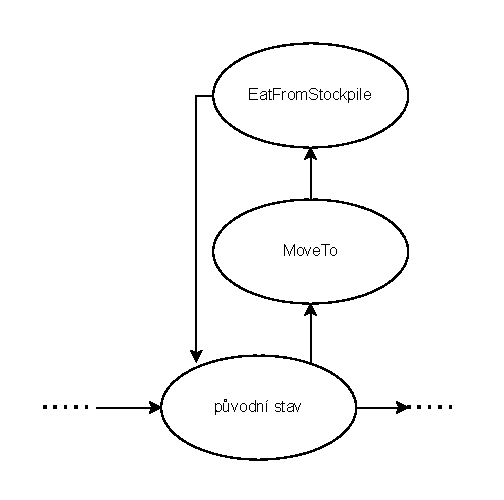
\includegraphics[width=0.6\linewidth]{img/transition.pdf}
    \caption{Řešení mechaniky hladu pro jeden vrchol z původního stavového automatu.}
    \label{fig:transition}
\end{figure}

Alternativní způsob by byl použít dva stavové automaty. Hlavním automatem by byl automat řešící hlad, který by měl \texttt{MainState} ve kterém by se nejprve zkontrolovalo zda hladovění vesničana nekleslo pod určitou hodnotou, pokud ne tak zavolá původní automat, jinak nastane přechod do již zmiňované dvojice stavů \texttt{MoveToState} a \texttt{EatFromStockpileState}.

Je lehké nahlédnout, že obě řešení přidávají netriviální složitost navíc do definice chování pro naše vesničany.

Podle výše zmíněného článku mají \textit{stromy chování} dobrou rozšiřitelnost a modularitu. Pokud bychom chtěli rozšířit náš \textit{strom chování} o výše zmíněnou mechaniku hladu, mohli bychom vytvořit nový strom chování, který by použil \texttt{Selector} vrchol jako kořen, který by měl dva potomky. Prvním by byl podstrom řešící mechaniku hladu a druhým by byl celí původní strom připojený kořenem jako podstrom nového stromu chování. Celá situace by vypadala takto:

\begin{verbatim}
    Builder.Create()
      .Selector("tree root")
        .Sequence("villager hunger sequence")
          .Condition("is hunger bellow threshold?", IsHungry)
          .Condition("is there food?", IsThereFood(stockpile))
          .Do("go to get food", MoveTo(stockpile))
          .Do("eat food", EatFood)
        .End()

        .Sequence("villager job sequence")
          // original tree as subtree
        .End()
      .End()
\end{verbatim}

Je lehké nahlédnout, že rozšiřitelnost a modularita \textit{stromů chování} jsou opravu silné vlastnosti. Proto také \textit{stromy chování} použijeme pro definici chování pro naše vesničany.


\section{Generovaný svět}
\label{sec:terrain}
Jak jsme si specifikovali v sekci~\ref{sec:game-world}, svět v naší hře bude náhodně generovaný. Konkrétně bude obsahovat náhodně generovaný terén ve kterém budou náhodně umístěny suroviny a vesnice.

Vygenerovaný terén bude 2D plocha, která se bude skládat ze spojitých oblastí. Každá oblast bude odpovídat nějakému biomu a bude mít barvu podle tohoto biomu (například oblast odpovídající biomu vody bude modrá). Některé oblasti mezi sebou budou mít závislosti (například oblast, která reprezentuje biom vysoké hory, bude obklopena oblastí, která reprezentuje biom hory). Je nutné zmínit, že nechceme políčka, ale opravdu spojité oblasti.

Naši hru budeme používat převážně pro měření výkonu ECS knihoven, tím pádem nemáme na generování našeho terénu žádné složité požadavky. Mezi naše požadavky patří:

\begin{enumerate}
    \item \textbf{Generování terénu by nemělo trvat příliš dlouho:} Pokud by generování terénu trvalo příliš dlouho, vedlo by to k delšímu času spouštění naší hry. Vzhledem k tomu, že hru budeme používat pro měření výkonu ECS knihoven a pro každou knihovnu ji pouštět znovu, delší čas spouštění hry by nám zbytečně natahoval dobu vykonávání jednoho měření.

    \item \textbf{Možnost navigace:} Ze sekce~\ref{subsec:villages} víme, že hra bude obsahovat vesničany. Pro vesničany bude důležité aby byli schopni se v náhodně vygenerovaném terénu navigovat. Pokud vesničan bude například chtít jít pokácet strom, bude se chtít po cestě k němu vyhnout vodě.

    \item \textbf{Žádné vizuální artefakty:} Chceme se vyhnout vizuálním artefaktům, díky kterým by náš terén nevypadal dobře.
\end{enumerate}

\subsection{Generování terénu}
\label{sec:terrain-gen}
Z požadavků na naši hru, které jsme si představili v sekci~\ref{sec:game-characteristics} vyplývá, že nechceme naši hru dělat příliš složitou. Terén tedy budeme generovat tím, že si za pomoci šumové funkce nejprve vytvoříme výškovou mapu a tu poté obarvíme. Tento přístup jsme zvoli jelikož je jednoduchý na implementaci a poskytuje dobře vypadající terén.

Pro vygenerování výškové mapy bude nejprve nutné zvolit šumovou funkci, proto si jednotlivé šumové funkce nejprve rozebereme:

\begin{enumerate}
    \item \textbf{Perlinův šum:} Jedná se o známou šumovou funkci. Tato šumová funkce je rychlá a také jednoduchá na implementaci. Je jí možné použít v libovolné dimenzi, ale nejčastěji se používá ve druhé nebo třetí. Přehledné vysvětlení o tom co to je Perlinův šum a jak se používá pro generování terénu je možné nalézt v diplomové práci \textit{Terrain synthesis using noise}~\cite{TerrainNoise} od \textit{Tuoma Hyttinena}.

    \item \textbf{Simplexový šum:} \textit{Simplexový šum} je velmi podobný \textit{Perlinovu šumu}. Přehledné vysvětlení o tom co to je \textit{Simplexový šum} a jak se používá pro generování terénu je možné nalézt v již zmíněné diplomové práci \textit{Terrain synthesis using noise}~\cite{TerrainNoise}. V této práci je možné se dočíst, že oproti \textit{Perinovu šumu} je \textit{Simplexový šum} rychlejší a produkuje výsledky, které vypadají více přirozeně. Ovšem má jednu velkou nevýhodu a to patent, který omezuje jeho použití pro komerční účely. Z toho důvodu se v praxi tolik nepoužívá.
\end{enumerate}

I přesto je \textit{Simplexový šum} nabízí výhody oproti \textit{Perlinovu šumu}, pro implementaci zvolíme \textit{Perlinův šum} z důvodů již zmíněného patentu. Konkrétně jej budeme používat ve druhé dimenzi.

Nyní za pomoci \textit{Perlinova šumu} vygenerujeme výškovou mapu. Pro generování výškové mapy lze použít Fraktální součet nebo TurbulencI. Jedná se o techniky pro generování více komplexních vzorů. O obou technikách je možné se více dočíst v již zmíněné diplomové práci \textit{Terrain synthesis using noise}~\cite{TerrainNoise}.

Pro zvolení techniky autor práce provedl experiment a nechal vygenerovat terén pomocí obou technik. Z výsledných terénů autor více preferoval terén vygenerovaný Fraktálním součtem, proto jej zvolíme.

Nyní zbývá pomocí výškové mapy vygenerovat daný terén. Již víme, že náš terén bude 2D plocha. Tuto plochu si rozdělíme na malé atomické části (například pixely) a těmto částem přiřadíme souřadnice. Barva každé části bude odpovídat danému biomu. Každý biom bude mít definovaný výškový interval a barvu. Pro souřadnice každé atomické části si necháme vygenerovat výšku z výškové mapy. Poté na základě této výšky a výškových intervalů jednotlivých biomů získáme příslušný biom. Poté barvu dané části nastavíme na barvu daného biomu. O této technice je možné se více dočíst ve článku \textit{Making maps with noise functions}~\cite{TerrainHeightMap} ze stránky \textit{Red Blob Games}.

Příklad výsledného terénu je možné vidět na obrázku~\ref{fig:terrain}.

\begin{figure}[!htb]
    \centering
    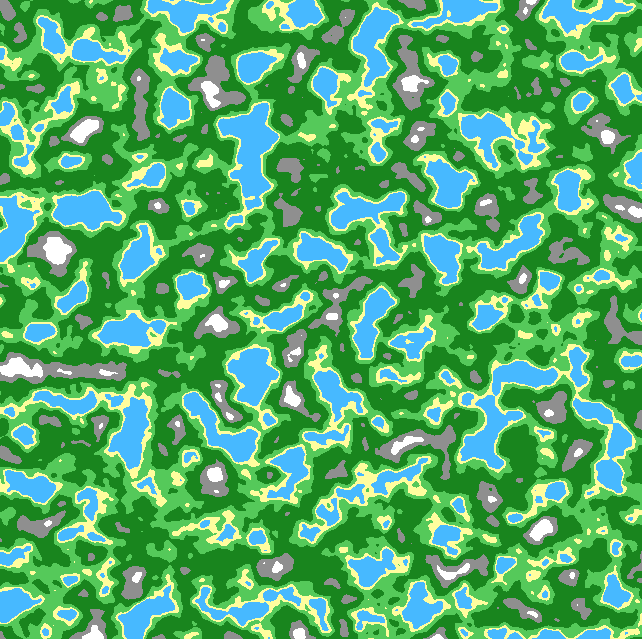
\includegraphics[width=0.66\linewidth]{img/terrain.png}
    \caption{Příklad jak může vypadat námi vygenerovaný terén.}
    \label{fig:terrain}
\end{figure}

\subsection{Generování terénu na CPU vs. GPU}
Za použití techniky z minulé sekce jsme získali vygenerovaný terén. Ovšem to jestli naše technika splňuje naše požadavky je závislé na tom zda terén budeme generovat na CPU nebo na GPU. Proto si nyní oba přístupy rozebereme.

\subsubsection{Generování terénu na CPU}
Při generování terénu na CPU bychom si pořídili jednu nebo více textur a vygenerovali terén v nich za použití způsobu z minulé sekce.

Při generovaní tohoto terénu je možné zvolit rozlišení, konkrétně specifikaci velikosti atomických částí. Volba tohoto rozlišení nám ovlivňuje dobu trvání vygenerování našeho terénu. Pokud bychom zvolili malé atomické části, generování by trvalo příliš dlouho a porušili bychom požadavek na rychlost. Pokud bychom zvolili velké atomické části, generování by trvalo menší dobu, ale zase bychom porušili požadavek na absenci vizuálních artefaktů.

V ideálním případě bychom chtěli velké rozlišení ale také lepší rychlost. Jeden ze způsobů jak toho dosáhnout je paralelizace, ovšem možnosti paralelizace na CPU jsou oproti GPU omezeny, proto si rozeberme jak by se dal terén generovat na GPU.

\subsubsection{Generování terénu na GPU}
Terén budeme generovat v reálném čase (vygenerujeme jej v každém snímku znova) a vždy nám postačí vygenerovat pouze část terénu, která je viditelná hráčem. Tato část bude bude obdélník se stejnými rozměry jako velikost okna naší hry.

Pořídíme si texturu do které budeme generovat terén. Tato textura bude mít stejnou velikost jako okno naší hry. Poté si pořídíme fragment shader, kterým do této textury budeme generovat terén. Tento fragment shader v každém snímku na základě pozice a přiblížení kamery pro každý pixel naší textury provede algoritmus popsaný v sekci~\ref{sec:terrain-gen}.

Díky vysoké paralelizaci GPU můžeme vždy zvolit nejmenší velikost atomických oblastí (velikost jednoho pixelu) a stejně budeme mít pořád dostatečnou rychlost.

\subsection{Navigace ve vygenerovaném terénu}
Generování terénu na GPU se zdá být ideálním kandidátem, ovšem tím, že terén budeme generovat na GPU, nám vzniká problém, jak ve vygenerovaném terénu budeme vlastně provádět navigaci. V této sekce tento problém vyřešíme.

Vesničané v naší hře budou často potřebovat nalézt cestu v námi vygenerovaném terénu k nějaké entitě. Budou například chtít dojít ke skladišti nebo ke svému pracovnímu místu. Jelikož k hledaní cesty bude docházet poměrně často budeme chtít aby bylo dostatečně rychlé. Dále budeme chtít, aby cesty působily přirozeně. Příklady vhodných (přirozených) a nevhodných (nepřirozených) cest je možné vidět na obrázku~\ref{fig:path}.

\begin{figure}[!htb]
    \centering
    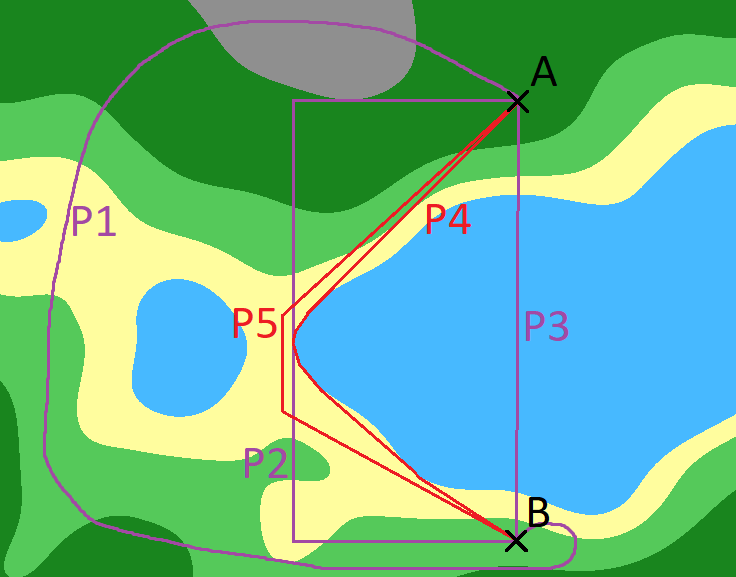
\includegraphics[width=0.66\linewidth]{img/path.png}
    \caption{Příklad cest z bodu A do bodu B. Fialové cesty jsou nevhodné. Červené cesty jsou vhodné.}
    \label{fig:path}
\end{figure}

Fialové cesty jsou nevhodné. Konkrétně cesta $P1$ je nevhodná, jelikož vede zbytečnou velkou oklikou. Cesta $P2$ je nevhodná, protože vede pouze podel os. Cesta $P3$ je nevhodná, jelikož vede přes vodu.

Červené cesty jsou vhodné. Cesta $P4$ je nejkratší cestou z bodu $A$ do bodu $B$. Cesta $P5$ sice není nejkratší cesta ale je pro nás dostatečně dobrou aproximací a je pro nás dostačující.

\subsubsection{Navigační struktury}
Pro navigaci v terénu použijeme datovou strukturu. Tato datová struktura reprezentuje terén způsobem, který umožňuje snadné hledaní cest mezi dvěma body. Často k tomu používají algoritmus pro hledání nejkratších cest. Typickou volbou bývá algoritmus A*. Datové struktury, které lze pro navigaci použít nazvěme navigační struktury.

Velkou část navigačních struktur tvoří navigační meshe (nebo také zkráceně navmesh). Ty jsou často používány populárními frameworky a enginy jako je například Unity. Navigační meshe vezmou plochu terénu po které lze chodit a rozdělí ji do oblastí. Každá taková oblast je tvořena konvexním polygonem. Poté si vytvoří graf, kde každý takovýto polygon je reprezentován vrcholem a každé sousední polygony mají mezi sebou hranu. V tomto grafu se poté hledají nejkratší cesty. Je nutné upozornit, že existuje velké množství navigačních meshů a některé se od tohoto popisu mouhou lišit. Pro více informacích o navigačních meshích lze nahlédnou do studie \textit{A comparative study of navigation meshes}~\cite{10.1145/2994258.2994262}.

V sekci~\ref{sec:game-characteristics} jsme si uvedli, že nechceme aby naše hra byla příliš složitá, jelikož by to odvádělo pozornost od problému, který řešíme. Z toho důvodu nebudeme používat navigační mesh jako navigační strukturu pro naši hru, jelikož i přesto, že použití navigačního meshe pro navigaci není složitá úloha tak jeho konstrukce složitá já.

Jako navigační strukturu zvolíme dvourozměrnou mřížku. Tu si budeme reprezentovat jako pole, kde každý prvek tohoto pole ponese informaci o tom v jakém biomu se nachází daný vrchol mřížky. Tuto strukturu zvolíme, protože je jednoduchá na konstrukci. Cesty které díky této mřížce získáme nebudou nejlepší možnou nejkratší cestou (a nebudou ve skutečnosti ani nejkratší), ale budou pro nás dostatečně dobrou aproximací. 

\subsubsection{Tvorba cesty}
Tvorbu cesty začneme tím, že získáme cestu, která se bude z počátku nevhodná. Poté ji vylepšíme a tím získáme cestu, která již bude vhodná.

Pro výpočet vzdálenosti mezi dvěma body v naší mřížce zvolíme Manhattanskou metriku. Pro hledání nejkratších cest použijeme algoritmus A*. První tvar naší cesty získáme tím, že pomocí A* algoritmu nalezneme cestu v naší mřížce. Příklad toho jak by taková cesta mohla vypadat je možné vidět na obrazku~\ref{fig:path_grid}. Je lehké nahlédnout, že se podobá cestě $P2$ z obrázku~\ref{fig:path}, která je pro nás nevhodná.

\begin{figure}[!htb]
    \centering
    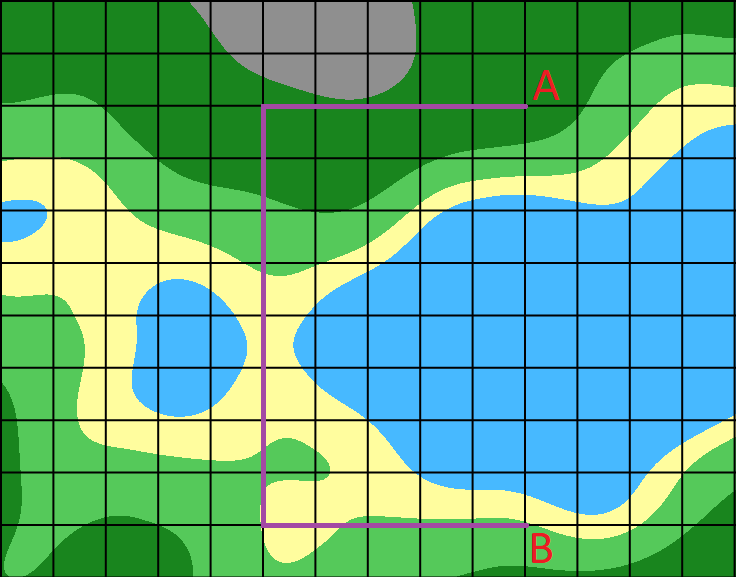
\includegraphics[width=0.66\linewidth]{img/path_grid.png}
    \caption{Příklad cesty z bodu A do bodu B nalezené A* algoritmem v naší mřížce.}
    \label{fig:path_grid}
\end{figure}

Následně provedeme úpravu této cesty.Začneme v prvním bodu cesty a provedeme ray cast do druhého bodu. Pokud jsme nenarazili na vodu pokusime se provést ray cast ke třetímu bodu. To budeme opakovat dokud náš ray cast nenarazil na vodu. V takovém případě můžeme cestu zjednodušit a odstranit z ní všechny body mezi prvním a posledním úspěšným. Poté ce přesuneme ke druhému bodu a postup opakujeme. Celí tento proces provádíme dokud nedojdeme do posledního bodu naší cesty. Zjednodušení fialové cesty je možné vidět na obrázku~\ref{fig:path_simplified}, kde fialová cesta představuje původní cestu a červená cesta její zjednodušení.

\begin{figure}[!htb]
    \centering
    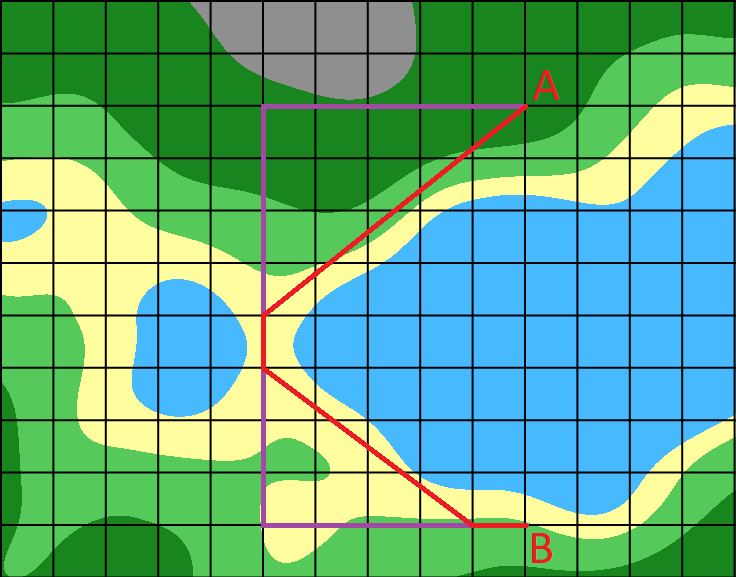
\includegraphics[width=0.66\linewidth]{img/path_simplified.png}
    \caption{Příklad cesty z bodu A do bodu B nalezené A* algoritmem v naší mřížce, která byla následně zjednodušena. Fialová cesta je originální nevhodná cesta. Červená cesta je zjednodušená, již vhodná, cesta.}
    \label{fig:path_simplified}
\end{figure}

Ovšem problém spočívá v tom, že k dispozici máme pouze mřížku, která obsahuje data o našem terénu, tím pádem nemůžeme provést klasický ray cast. Proto provedeme pouze jeho aproximaci. Začneme v bodu $N$ a chceme provést aproximaci ray castu do bodu $M$. Spočítáme si směr z bodu $N$ do bodu $M$ a tímto směrem se budeme posouvat vždy o nějakou malou vzdálenost $\Delta$. Pokaždé když se posuneme tak si spočítáme nejbližší bod z naší mřížky. Pokud se jedná o bod s biomem vody, tak ray cast selhal. V případě, že jsme takto došli až do bodu $M$ a nenarazili jsme na bod vody, ray cast byl úspěšný.

Mohlo by se zdát, že použití této aproximace by vedlo v příliš nevhodné cesty, ovšem za předpokladu, že se body v naší mřížce budou nacházet dostatečně blízko sebe, tak bude výsledná cesta dostatečně dobrou aproximací červené cesty z obrázku~\ref{fig:path_simplified}.

Další problém, který je nutné vyřešit, je, že vesničané a entity, ke kterým se vesničané navigují, nejsou umístěni v naší mřížce. Problém vyřešíme tak, že před spuštěním A* algoritmu si k vesničanovi a dané entitě nalezneme nejbližší body v naší mřížce a nalezneme nejkratší cestu mezi těmito body. Poté, předtím než provedeme zjednodušení cesty, přidáme pozici vesničana jako první bod naší cesty a pozici entity, ke které se vesničan naviguje, jako poslední bod naší cesty. Přidáním těchto bodů by nám mohli vzniknout nepřirozené artefakty, ovšem ty budou spraveny během zjednodušování cesty.

Zbývá nám vyřešit jak získáme již zmiňovanou mřížku. Abychom ji získali z našeho terénu bude potřeba jej navzorkovat. Podobně jako při jeho generování si terén rozdělíme na atomické části a střed každé takové atomické části bude bodem v naší mřížce. Protože celý náš terén generujeme na GPU, bude nutné toto navzorkování také provádět na GPU. Pořídíme si proto compute shader pomocí kterého terén navzorkujeme na GPU a tím vytvoříme mřížku, kterou poté přesuneme na CPU.

Ovšem problém nastává v tom, že MonoGame framework, který pro tvorbu naší hry používáme nemá podporu pro compute shadery. Z toho důvodu namísto nativního MonoGame zvolíme jeho fork~\cite{MonoGameCptMax} od Markuse Hötzingera, který tuto podporu přináší.

\section{Měření}
\label{benchmark-analysis}
Z úvodu této kapitoly víme, že náš projekt je reprezentován C\# řešením. Toto C\# řešení se skládá ze dvou C\# projektů a to hry a poté měření, které používá onu hru pro měření výkonu ECS knihoven. V této sekci se budeme věnovat analýze tohoto měření.

\subsection{Jak budeme měření provádět}
Prvně si přiblížíme co to je \textit{game loop}, jelikož to budeme potřebovat k popisu měření. Následně si popíšeme samotné měření.

\subsubsection{Game loop}
\label{game-loop}
\textit{game loop} si můžeme představit jako cyklus, který běží dokud nedojde k ukončení hry. Pseudokód pro \textit{game loop} může vypadat například takto:

\begin{verbatim}
    while (!shouldExit) 
    {
      Update();
      Draw();
    }
\end{verbatim}

Pseudokód obsahuje \texttt{while} cyklus, který se opakuje dokud nedojde k nastavení proměnné \texttt{shouldExit} na \texttt{true}. V těle tohoto cyklu se volají dvě funkce a to \texttt{Update}, která je zodpovědná za zpracování herní logiky a \texttt{Draw}, která je zodpovědná za vykreslení hry. 

I naše hra obsahuje \textit{game loop}. Logika v naší hře se skládá ze systémů. Ty se dělí na \textit{update systémy}, které řeší zpracování herní logiky a \textit{render systémy}, které řeší vykreslování. \textit{Update systémy} běží uvnitř funkce \texttt{Update} a \textit{render systémy} běží uvnitř funkce \texttt{Draw}. Je nutné upozornit, že tento popis je zjednodušen a více dopodrobna se implementaci hry a systémů budeme věnovat v následující kapitole.

\subsubsection{Popis měření}
Budeme mít stanovené dva pevné počty iterací. První bude přípravný počet iterací a druhý bude měřený počet iterací. Měřený počet iterací bude větší než přípravný počet iterací.

Samotné měření se bude skládat ze dvou fází a to fáze přípravy a fáze měření. Během fáze přípravy vytvoříme instanci naší hry s konkrétní ECS knihovnou a necháme její \textit{game loop} běžet přípravný počet iterací. Během fáze měření vezmeme tu samou instanci hry, která běžela přípravný počet iterací a necháme její \textit{game loop} běžet měřený počet iterací. Během fáze měření budeme také měřit čas, během kterého hra provádí měřený počet iterací svého \textit{game loop}. Tento čas bude výsledným časem pro jednu konkrétní ECS knihovnu.

Výše popsaný test provedeme pro každou ECS knihovnu, kterou budeme měřit. Pomocí výsledných časů můžeme relativně porovnat výkon naší hry s různými ECS knihovnami. 

Při měření výkonu jednotlivých ECS knihoven ignorujeme některé jejich funkcionality. Konkrétně se jedná o funkcionality rozšíření ECS. Jedná se například o funkcionality známe pod názvy \textit{reakční systémy} (\textit{reaction systems}) nebo \textit{relace} ({\textit{relations}}). V našem měření je budeme ignorovat protože chceme měřit klasické ECS bez rozšířeních.

\subsection{Volba frameworku pro měření}
\label{benchmark-framework}
Nyní zvolíme framework, který budeme používat pro měření. Prvně si popíšeme vlastnosti, kterého od tohoto frameworku požadujeme, poté provedeme samotný výběr. Mezi požadované vlastnosti patří:

\begin{enumerate}
    \item \textbf{Korektnost:} Chceme aby naměřené výsledky byli spolehlivé. Klíčovým faktorem bude aby výsledek vyprodukovaný pro danou ECS knihovnu byl porovnatelný s výsledkem vyprodukovaným pro jinou ECS knihovnu.
    \item \textbf{Jednoduchost:} Budeme chtít aby framework byl jednoduchý na používání. Nechceme dávat přednost jednoduchosti před korektností, ale pokud bude na výběr mezi frameworky co splňují první požadavek, tak upřednostníme ten, který je jednodušší na používání.
\end{enumerate}

Pro výběr frameworku použijeme platformu GitHub. Na stránce~\cite{github_performance} je možné vidět seznam repositářů na platformě GitHub s topicem \textit{performance} seřazené podle počtu hvězd. Je možné nahlédnou, že nejpopulárnějším frameworkem pro měření výkonu je \textit{BenchmarkDotNet}~\cite{BenchmarkDotNet}.

\textit{BenchmarkDotNet} je framework pomocí kterého lze měřit výkon metody. Tento framework splňuje oba naše požadavky, ale jedná se o framework primárně určený na micro benchmarky, zatímco naše měření je spíše macro benchmarkem. I přesto jej pro naše měření použijeme, primárně protože je velmi jednoduchý na použití.

















% \subsection{Jak lze měřit výkon hry}
% Pro měření výkonu budeme mít test, který si pro každou ECS knihovnu, kterou budeme měřit, vytvoří novou instanci naší hry běžící s danou ECS knihovnou. Poté tento test změří výkon každé takovéto instance. Ještě předtím, než si rozebereme přístupy pro měření výkonu hry si nejprve připomeneme co to je \textit{game loop}.

% \subsubsection{Game loop}
% \textit{game loop} si můžeme představit jako cyklus, který běží dokud nedojde k ukončení hry. Pseudokód pro \textit{game loop} může vypadat například takto:

% \begin{verbatim}
%     while (!shouldExit) 
%     {
%       Update();
%       Draw();
%     }
% \end{verbatim}

% Pseudokód obsahuje \texttt{while} cyklus, který se opakuje dokud nedojde k nastavení proměnné \texttt{shouldExit} na \texttt{true}. V těle tohoto cyklu se volají dvě funkce a to \texttt{Update}, která je zodpovědná za zpracování herní logiky a \texttt{Draw}, která je zodpovědná za vykreslení hry. 

% I naše hra obsahuje \textit{game loop}. Logika v naší hře se skládá ze systémů. Ty se dělí na \textit{update systémy}, které řeší zpracování herní logiky a \textit{render systémy}, které řeší vykreslování. \textit{update systémy} běží uvnitř funkce \texttt{Update} a \textit{render systémy} běží uvnitř funkce \texttt{Draw}. Je nutné upozornit, že tento popis je zjednodušen a více dopodrobna se implementaci hry a systémů budeme věnovat v následující kapitole.

% \subsubsection{Přístupy k měření výkonu}


% Nyní si rozebereme přístupy, kterými lze měřit výkon naší hry.

% co si od toho predstavujeme, jak to chceme delat

% vyber frameworku pro mereni

% na co nebudeme brat ohledy a proc









% První si popíšeme kde tuto mřížku vezmeme a poté jak ji budou využívat vesničané pro navigaci.

% Abychom získali z našeho terénu mřížku bude třeba jej navzorkovat. Podobně jako při jeho generování si terén rozdělíme na atomické části a střed každé takové atomické části bude bodem v naší mřížce. Ovšem celý náš terén generujeme na GPU, proto toto navzorkování bude nutné také provést na GPU. Pořídíme si proto compute shader pomocí kterého terén navzorkujeme na GPUa tím vytvoříme mřížku, kterou poté stáhneme do CPU.

% Ovšem problém nastává v tom, že MonoGame framework, který pro tvorbu naší hry používáme nemá podporu pro compute shadery. Z toho důvodu namísto nativního MonoGame zvolíme jeho fork~\cite{MonoGameCptMax} od Markuse Hötzingera, který tuto podporu přináší.




% \xxx{TODO: path-finding}

% Naše hra bude obsahovat procedurálně generovaný terén. Ten je možné generovat pomocí CPU nebo pomocí GPU. Obě možnosti si nyní rozebereme.

% % \subsubsection{Generování terénu na CPU}
% Při generování terénu na CPU nám postačí terén vygenerovat pouze jednou při spuštění hry a výsledek si poté uložit do jedné nebo více textur. Tento přístup má ale dva problémy. Prvním problémem je, že pokud dojde k většímu přiblížení nebo oddálení kamery, dojde k deformaci těchto textur. To může způsobit různé vizuální artefakty. Druhým problémem je, že vytváření zmíněných textur může trvat delší dobu. To může vést k delšímu času spouštění hry.

% % \subsubsection{Generování terénu na GPU}
% Pro vygenerování terénu na GPU ja potřeba vytvořit shader. Tento shader vezme pozici a přiblížení kamery a vygeneruje pro tyto parametry terén. Díky vysoké paralelizace na GPU můžeme terén generovat za běhu. Při generování terénu za běhu nám nevzniknou výše zmíněné vizuální artefakty. Vyřeší se nám i druhý problém, jelikož nemusíme čekat na vygenerování výše zmíněné textury.

% Je snadné nahlédnout, že generování terénu na GPU je pro nás výhodnější, proto tento přístup zvolíme.

% \section{Hledání cesty ve vygenerovaném terénu}
% \label{subsection:path-finding}
% Vesničané musejí často vyhledávat cestu z bodu A do bodu B. Například potřebují dojít ke svému pracovnímu místu, nebo odnést předmět do skladiště.

% V případě generování terénu na CPU by bylo hledání cesty velice jednoduché. Stačilo by nám vzít vygenerovanou texturu a najít danou cestu v ní. Ovšem problém spočívá v tom, že terén generujeme pomocí GPU a vyhledávání cesty musíme vykonávat na CPU.

% Pro řešení problému s hledáním cesty si zavedeme \textit{compute shader}, který jako vstupní parametr přijme rozlišení. Výstupem tohoto \textit{compute shaderu} bude dvourozměrné pole sestavené z nevzorkovaného terénu při daném rozlišení. Tento \textit{compute shader} nám tedy při spuštění hry vytvoří dvourozměrné pole na GPU, to si poté stáhneme na CPU a v něm poté můžeme provádět vyhledávání cesty.

% Chceme pěkné cesty, takže výslednou cestu zkrášlujeme.

% Generování může trvat, protože přesun dat mezi GPU a CPU je drahý.

% Je nutné použít fork MonoGame, který podporuje compute shadery.

% \section{Owner komponenta}
% Při práci s ECS je někdy potřeba získat identifikátor příslušné entity. Ovšem v kontextu systému, který pouze iteruje přes komponenty na jednotlivých entitách to může být problematické.

% Řešení, které některé ECS knihovny nabízejí je možnost iterovat identifikátory entit společně s jejich komponentami. Ovšem ne každá ECS knihovna to umí, proto je potřeba zvolit jiný přístup.

% Přístup, který jsme zvolili je zavedení \texttt{Owner} komponenty. Jednotlivé entity jsou v naší hře reprezentovány třídou dědicí od \texttt{IEntity}. \texttt{Owner} komponenta má pouze jeden jediný člen a to referenci na \texttt{IEntity}, která představuje jejího majitele.









% \subsection{Reprezentace systémů}
% Jak již bylo zmíněno v úvodu, velký problém při návrhu systémů je rozdílné rozhrani, které pro systémy jednotlivé ecs knihovny nabízejí.

% Dále, jak již jsme si zmiňovali v podkapitole o herních požadavcích, chceme aby se výkon naší hry při použití této abstrakční vrstvy blížil výkonu s použitím pouze samotné ecs knihovny.

% Nahlédneme na oba tyto problémy blíže a prozkoumáme jak jsme je vyřešili.

% \subsubsection{Rozhraní ecs knihoven}
% ECS knihovny reprezentují systémy následujícími způsoby:

% \begon{ordering}
% \item \xxx{TODO}
% \end{ordering}











% V této sekci si představíme knihovny, které budeme chtít měřit. Nahlédneme na jejich rozhraní a na základě toho odůvodníme rozhodnutí provedené při implementaci abstrakční vrstvy.

% % - knihovny
% \subsection{Měřené knihovny}
% Než začneme provádět analýzu abstrakční vrstvy, musíme si nejprve představit jednotlivé knihovny, které budeme chtít měřit. Následně nahlédneme na jejich rozhraní, to nám pomůže při analýze abstrakční vrstvy.

% % --- predstaveni knihoven
% I přesto, že lze program použít pro měření velkého množství ECS knihoven pro C\#, omezíme se pouze na následující:

% \begin{enumerate}
%     \item Arch~\cite{Arch}
%     \item DefaultEcs~\cite{DefaultEcs}
%     \item Entitas~\cite{Entitas}
%     \item HypEcs~\cite{HypEcs}
%     \item LeoECS~\cite{LeoECS}
%     \item \xxx{Pridat dalsi knihovny kdyz bude cas.}
% \end{enumerate}

% \xxx{ --- rozebrat interface knihoven}\\\\

% \section{Inline entity processor}

% Inlinování funkcí je optimalizace, při které je volání funkce nahrazeno jejím obsahem.

% % priklad, kdy dochazi k inlinovani

% Kvůli měření je důležité, aby naše entity procesory neměli ideálně žádný overhead.

% Pro inlinování entity procesorů, využíváme následující techniky.

% % aggressive inlining, struktura + generika

% % \\
% % \xxx{Proc je to potreba}
% % \\
% % \xxx{Jak jsme toho dosahli}
% % \\

% \xxx{ - entity processor}\\\\
% \xxx{ --- -> entity processor}\\\\
% \xxx{ --- co je inline function call}\\\\
% \xxx{ --- jak jej zaridit}\\\\
% \xxx{ --- -> proto struktura a generika (IECSSystem)}\\\\

% \xxx{ - IEntity (chceme bohate rozhrani, jak jsme si popisovali)}\\\\
% \xxx{ - IWorld (nektere ECS knihovny potrebuji Update/Tick)}\\\\
% \xxx{ - Component attribute}\\\\
% \xxx{ - ECSFactory (proc types - zjednoduseni rozhrani)}\\\\

% \section{Analýza hry}

% text

% \subsection{Implementace AI}

% Nyní si rozebereme populární přístupy pro implementaci AI ve hrách.

% Nejpřímočařejší způsob je použít stavové automaty.

% Pokročilejší zpusob jsou behavior trees.

% Další pokročilejší způsob je Goal Oriented Action Planning (GOAP).

% Proč jsme zvolili behavior trees?

% Chování AI agentů může být popsané také přímo v systémech.

% Ne vždy je zřejmé co by mělo být součástí AI.

% \\
% \xxx{jaka jsou mozsnosti?}
% \\
% \xxx{- behavior trees}
% \\
% \xxx{- state machines}
% \\
% \xxx{- GOAP}
% \\
% \xxx{proc jsme zvolili behavior trees?}
% \\
% \xxx{behavior primo v systemech a proc jsme to nepouzili}
% \\
% \xxx{Co by melo byt rizeno AI a co ne?}
% \\
% \xxx{- tezba surovin: pripsani do inventare vs damage and drop system}
% \\
% \xxx{- zpracovani surovin: pripsani do inventare vs resource processing system}
% \\

% \subsection{ECS}

% Některé systémy v ECS reagují pouze pokud je pro danou entitu splněna určitá podmínka.

% Na první pohled by se mohlo zdát, že jsou tyto systémy špatné, jelikož podmínka je drahá operace.

% Alternativní a pravděpodobně lepší způsob je použít eventy.

% Rozeberme si jak by se s eventy v ECS pracovalo.

% Další způsob, jak by se tento problém dal řešit jsou Reaction systémy.

% \\
% \xxx{condition checking systems are ok}
% \\
% \xxx{eventy v ECS}
% \\

% \subsection{Generovani terenu}

% Rozeberme si dva přístupy pro generování terénu.

% První způsob je generovat terén přímo na CPU.

% Druhý způsob je pro generování terénu použít GPU.

% problem s path finding

% Abychom si rozebrali řešení, bude nejprve nutné nejprve  něco více o shaderech.

% Compute shader můžeme použít k řešení výše zmíněného problému.

% \xxx{GPU vs CPU}